%% HBM
%%

\subsection{Calibration Data}

For our calibration data, we used a sample of \Kepler\ stars with
both asteroseismic and flicker measurements available. \citet{chaplin:2014}
report asteroseismic \rhostar\ estimates (and the associated uncertainties) for
518 \Kepler\ stars. The authors report three different sets of results,
depending on the choice of \Teff\ and \FeH, and in this work we elected to use
values reported in their Table 6 over Table 5, and Table 5 over Table 4. We
additionally used the 71 additional planet hosting stars with asteroseismology
reported in \citet{huber:2013} but not reported in \citet{chaplin:2014}. Values
for flicker and ``range'' were taken from \citet{kipping:2014}, based upon the
methods described in \citet{bastien:2013}. Following \citet{kipping:2014} and
for reasons described there-in, we only include targets in our calibration for
which:

\begin{itemize}
\item[{\tiny$\blacksquare$}] Range (defined in \citealt{bastien:2013})
$<1$\,ppt
\item[{\tiny$\blacksquare$}] $4500<T_{\mathrm{eff}}<6500$\,K
\item[{\tiny$\blacksquare$}] $K_P<14$
\item[{\tiny$\blacksquare$}] $1.2 < \log_{10}$($F_8$\,[ppm])$< 2.2$
\end{itemize}

We use the same sample for our calibration of \logg, except that we exclude the
\citet{huber:2013} data, since these authors do not provide estimates of
\logg\footnote{Whilst we could compute \logg\ ourselves from the reported
masses and radii, this could only be done under the incorrect assumption of
zero covariance between $M_{\star}$ and $R_{\star}$.}.

\subsection{Hierarchical Bayesian Model}

We model the stochastic relationship between $F_8$ and \logg\ or \rhostar,
accounting for the fact that there exists some intrinsic scatter in
the dependent variable, and including the heteroskedastic uncertainties on both
the dependent and independent variables.
There are two excellent reasons for modelling the relation stochastically;
firstly, if the intrinsic scatter is ignored and the relation between
variables is assumed to be deterministic, those data points with smaller
measurement uncertainties may have an unrepresentative greater weighting
during the fitting process \citep{hogg:2010b}.
Secondly, we are interested in producing probability distributions over stellar
densities and surface gravities, as opposed to point estimates, and propagating
these probability distributions through to subsequent analyses.
Several recent studies have required posterior Probability Distribution
Function (PDF) samples, in order to conduct their (hierarchical)
analyses \citep[e.g.][]{foreman-mackey:2014, rogers:2015, angus:2015}.

Including observational uncertainties on the independent variable within our
analysis is also important, because ordinary least squares regression methods
performed on data with two-dimensional uncertainties will result in a slope
that is biased towards zero
\citep[e.g.][]{fuller:1987, fox:1997}.
For a demonstration of the affects of neglecting intrinsic scatter and
two-dimensional uncertainties, see \citet{kelly:2007}.

We write the two models describing the relationship between $F_8$, \logg\ and
\rhostar\ as
\begin{equation}
	\log_{10}(\rho_\star) \sim \mathcal{N} \left(\mu = \alpha + \beta
	\log_{10}(F_8), \sigma = \sqrt{\sigma_{\rho}^2 + \gamma F_8}\right),
\end{equation}
\label{eq:rho}
and
\begin{equation}
	\log_{10}(g) \sim \mathcal{N}\left(\mu = \delta + \epsilon \log_{10}(F_8),
	\sigma = \sqrt{\sigma_g^2 + \zeta F_8}\right).
\end{equation}
\label{eq:logg}
The free parameters of the two models are $\alpha$, $\beta$, $\gamma$
$\sigma_{\rho}$, $\delta$, $\epsilon$, $\zeta$ and $\sigma_g$.
These relations are Gaussian distributions with means
given by the equation of a straight line, and standard deviations which
describe the intrinsic scatter about the mean as a function of flicker.

In order to account for the two-dimensional observational uncertainties in
this data set, we marginalize over the latent, `true' values of $F_8$,
\rhostar\ and \logg\ using the importance sampling method of
\citep{hogg:2010}\footnote{Note that while the pseudo-marginal MCMC method of
\citep{andrieu:2009} provides a truly unbiased estimate of the marginalized
likelhood, we expect any bias introduced by the importance sampling method to
be negligable.}.
In what follows we give an overview of this procedure, but encourage the
reader to refer back  to this original reference for a more detailed
description of the mathematics.
The observed values of the variables; $F_8$, \rhostar\ and \logg\ can be
thought of as a single `draw' from an underlying (assumed Gaussian)
probability
In what follows we give an overview of the importance sampling procedure, but
encourage the reader to refer back to the original reference for a more
detailed description of the mathematics.
The observed values of the variables; $F_8$, \rhostar\ and \logg\ can be
thought of as a single `draw' from an underlying (assumed Gaussian)
probability distribution, with mean equal to the `true' value---the value that
would have been observed, given infinitely high signal-to-noise---and standard
deviation equal to the observational uncertainty.
We compute the likelihood of the data given the model, marginalized over the
true values, using importance sampling.
We sample from the posterior PDFs of the true values of the variables,
conditioned on the observed values, and compute the likelihood of each of those
samples.
% These posterior PDFs could be produced by the astronomers who provide the
% catalog.
% If posterior samples are made available, they can be used in this stage of
% the inference.
% In the event that they are not provided however, they can be generated.
% For example, the $log(g)$ values used here are point estimates of the
% posterior PDFs of $log(g)$, produced by \citet{chaplin:2014} using
% {\it Kepler} light curves and stellar models.
We would use the posterior samples generated in previous model fitting process
if they were available, however generating new samples is an acceptable
approximation provided the posteriors are Gaussian and the priors used by the
previous fitters were uninformative.
Such an approximation will not be necessary for those studies using \rhostar\
or \logg\ calculated using the newly-calibrated relations presented here,
since we have published our posterior samples.
After producing new posterior PDF samples we then add up the individual
log-likelihoods of each sample to compute the total marginalized likelihood
for a star.
The marginalized likelihood of the whole dataset is then computed as the sum
of the log-likelihoods of each star.
The importance sampling method allows us to approximate the integral over the
latent variables.
% We used flat priors for all except the $\sigma$ parameters, for which we used
% priors which were flat in log-space.
We used uniform priors over all our parameters:
\begin{eqnarray}
	&	\alpha, \beta, \delta, \epsilon
	\sim U(-10:10) \\ \nonumber
 	&	\sigma_{rho}, \gamma, \sigma_g, \zeta  \sim U(-100:100).
\end{eqnarray}
\label{eq:priors}

We also performed this inference using an alternative, analytic form of the
marginal likelihood, which accounts for 2-D uncertainties but does not allow
the intrinsic scatter to be a function of the dependent or independent
variables.
For the relation between flicker and \rhostar, this likelihood function can be
written as
\begin{eqnarray}
	& p(\rho_*| F_8, \alpha, \beta, \sigma_{\rho}) =  \\ \nonumber
						      & \exp \left[-\frac{1}{2}
		\sum_{n=1}^N \frac{[F_{8n}-(\alpha + \beta \rho_{*n})]^2}
	{\left[\beta \sigma_{F8, n}^2 + (\sigma_{\rho *, n}
	+ \sigma_{\rho})^2\right]}\right]
	\\ \nonumber
	& + \beta^2 \sigma_{F8, n}^2 + (\sigma_{\rho *, n} + \sigma_{\rho})^2,
\end{eqnarray}
\label{eq:likelihood}
and similarly for \logg.
The parameter values found using this simple likelihood function are included
in table \ref{tab:results}.
% The analytic likelihood function, equation \ref{eq:likelihood} is suitable for
% cases where the intrinsic scatter is not a function of $x$ or $y$.
Figures \ref{fig:rhostar} and \ref{fig:logg} show the data with the best-fit
models.
The shaded regions show the 1 and 2$\sigma$ confidence interval which are
representative of the intrinsic scatter in the relations.
% Given a measurement of flicker, the predictive probability distribution of
% \logg and \rhostar will be a Gaussian distribution

%%% rhostar plot
\begin{figure}
\begin{center}
% \includegraphics[width=8.4cm,angle=0,clip=true]{../figs/rho_vs_flicker.pdf}
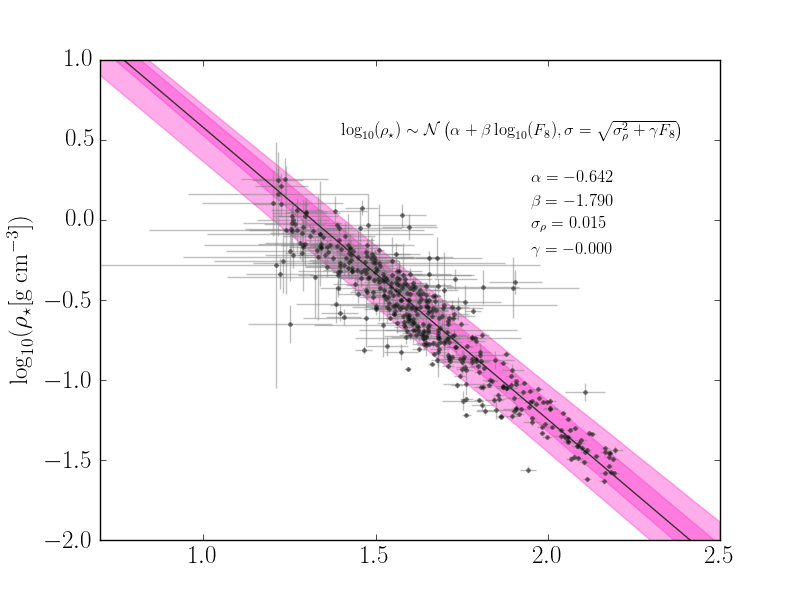
\includegraphics[width=8.4cm,angle=0,clip=true]{new_rho.pdf}
\caption{
Stellar density vs. flicker.
This figure shows the model, conditioned on the data.
The solid black line shows the highest-likelihood sample, and the pink shaded
regions show the 1 and 2$\sigma$ confidence intervals.}
\label{fig:rhostar}
\end{center}
\end{figure}

%%% logg plot
\begin{figure}
\begin{center}
% \includegraphics[width=8.4cm,angle=0,clip=true]{../figs/logg_vs_flicker.pdf}
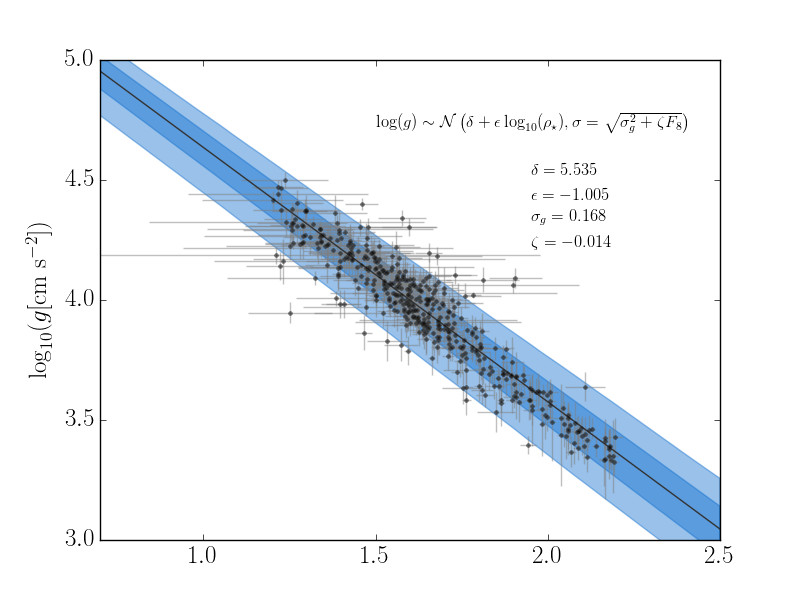
\includegraphics[width=8.4cm,angle=0,clip=true]{new_logg.pdf}
\caption{
$\log(g)$ vs. flicker.
As in \ref{fig:rhostar} this figure shows the model, conditioned on the data.
The solid black line shows the highest-likelihood sample, and the blue shaded
regions show the 1 and 2$\sigma$ confidence intervals.}
\label{fig:logg}
\end{center}
\end{figure}

\begin{table}
\caption{Highest-likelihood parameter values with 16th and 84th
	percentile uncertainties.}
\begin{tabular}{lccc}
\hline\hline
Parameter & highest-likelihood value & simple model result \\
    \hline
$\alpha$ &    2.358$_{-0.04}^{+0.08}$ &       2.191$_{-0.05}^{+0.05}$  \\
$\beta$ &    -1.79$_{-0.03}^{+0.04}$ &        -1.724$_{-0.03}^{+0.03}$ \\
$\sigma_{rho}$ &    0.015$_{-0.04}^{+0.08}$ &   0.085$_{-0.05}^{+0.05}$  \\
$\gamma$ &    -0.0$_{-0.04}^{+0.08}$ & \\
$\delta$ &    5.535$_{-0.07}^{+0.07}$ &      5.739$_{-0.03}^{+0.03}$  \\
$\epsilon$ &    -1.005$_{-0.04}^{+0.03}$ &   -1.095$_{-0.02}^{+0.01}$ \\
$\sigma_g$ &    0.168$_{-0.07}^{+0.07}$ &    0.015$_{-0.03}^{+0.03}$  \\
$\zeta$ &    -0.014$_{-0.07}^{+0.07}$ & \\
    \hline
\label{tab:results}
\end{tabular}
\end{table}
